\section{Preorder for combined non determinism and probabilities}

In this section we are going to fix a specific signature $\Sigma$
containing two binary operators $\prEff$ and $\orEff$. The two
operators are used to model a language where both probabilities 
and non-determinism coexist. Combining this specific effects has been 
the subject of numerous papers, and even when restricting ourselves to the 
denotational setting, the work of Regina Tix on powercones \cite{tix2009semantic} 
continued afterwards by Plotkin an Keimel \cite{KeimelP2016} on kegelspitze
shows the interest of such combination.
A more functional version of theses domains can also be found in the work of Jean-Goubault Larrecq 
\cite{JGL-mscs16}.

Given the recent developments of the denotational interpretation, 
it would be perfectly fine to use an interpretation 
to define our basic preorder $\sqeq_b$. But as we are studying 
operational semantics, it is more consistent to use an operational 
definition of the said preorder.

In the case of combined (demonic) non-determinism and probabilities we can define 
the preorder $\sqeq_b$ on trees over natural numbers in a simple and
effective way. We consider a tree as a Markov Decision Process 
and given an cost function from $\Nat \to \overline{\mathbb{R}_+}$
we find a strategy for the $\orEff$ nodes that minimizes the average
cost of the tree. 

A tree $t$ is under a tree $t'$ for this preorder when for any 
cost function, the minimal average cost for $t$ is under the 
minimal average cost for $t'$.

In order to formalise this intuition,
we define $\mathcal{S}$ to be the space representing 
the set of strategies. Given a strategy $s \in \mathcal{S}$ and 
a tree $t \in \Tree_\Nat$, one can build $t*s$ the application of 
the strategy to the tree, that builds a new \emph{probability} tree, that 
is \emph{without} $\orEff$ nodes. Given a probability tree, and a 
cost function $h$, one can define the expected cost as imagined. 
Now we can write:

\begin{equation*}
    t \sqeq_b t' \iff 
    \forall h : \Nat \to \overline{\mathbb{R}_+}, 
    \inf_{s \in \mathcal{S}} \mathbb{E}(h(t*s)) \leq 
    \inf_{s \in \mathcal{S}} \mathbb{E}(h(t'*s))
\end{equation*}

This preorder could be defined directly using Markov Decision Processes,
but in order to deduce the admissibility properties and the compositionality 
it is in our best interest to formalise in this slightly ad-hoc way.

Admissibility is going to rely on the \emph{scott-continuity} 
of the function $t \mapsto (h \mapsto \inf_{s \in \mathcal{S}} \mathbb{E} (h
(t*s)))$. Compositionality on the other hand is going to rely on an elementary 
decomposition result of the previous function.

\subsection{Formalisation of strategies} 

The goal of this subsection is to formalise strategies and 
to build a \emph{scott-continuous} function from $\Tree_\Nat \times \mathcal{S}$
to $\Tree_\Nat$ (without $\orEff$ nodes) corresponding to the 
application of a strategy to a tree.
First of all, because we know the shape of the trees, we can 
clearly define the set of strategies and recognise the Cantor 
Set, which has nice topological properties such as compactness.

\begin{adefinition}[Strategies]
     The set of strategies is 
     defined by $\mathcal{S} = \{ 0, 1 \}^\mathbb{N}$
     with the topology of the cantor space.
\end{adefinition}

\begin{ensps}
To define the probability following a strategy, we 
will first define how to modify a tree by applying a 
strategy to it. This corresponds to the intuitive 
idea that the strategy chooses a direction for every 
$\orEff$ node and leaves untouched any $\prEff$ node.
After such a transformation, the expectancy is going 
to be defined in a very easy and familial way because 
we will end up with a binary tree where each choice
has a probability one half.

Before defining application of a strategy to a tree,
lets first see a few functions over strategies 
that are continuous.

\begin{alemma}[Continuous functions over strategies]
    The following functions are continuous 
    \begin{enumerate}[(i)]
        \item $\drop : \mathcal{S} \to \mathcal{S}$ defined by $\drop(\alpha s) = s$
        \item $\odd : \mathcal{S} \to \mathcal{S}$ defined by $\odd((s_i)_i) = (s_{2i + 1})_i$
        \item $\even : \mathcal{S} \to \mathcal{S}$ defined by $\even((s_i)_i) = (s_{2i})_i$
    \end{enumerate}
\end{alemma}

Now that we have theses functions, we can define the space 
of strategies evaluations that are \emph{continuous}
functions from the cantor space to trees. 

This construction may seem unnatural, but it is the simplest 
way to get continuity of strategy application to a tree.

\begin{adefinition}[Application space]
    The space $\mathcal{C}(S,\Tree_\Nat)$ is a $\Sigma$-continuous 
    algebra where:

    \begin{enumerate}
        \item $\prEff (f,g) (\alpha s) = \prEff (f (\even(s)), g(\odd (s)))$ 
        \item $\orEff (f,g) (1 s)      = g(s)$
        \item $\orEff (f,g) (0 s)      = f(s)$
    \end{enumerate}
\end{adefinition}

Now that we have this space of function, we can define the 
homomorphism that maps a tree to a function from strategies 
to trees, that is the curryfication of the function we want to build.

\begin{adefinition}[Strategy Application]
    We define the function $*$ from $\Tree_\Nat$ to $\mathcal{C}(\mathcal{S},\Tree_\Nat)$
    as the unique homomorphism such that:

    \begin{enumerate}
        \item $n* = s \mapsto n$
        \item $\bot* = s \mapsto \bot$
    \end{enumerate}
\end{adefinition}

Note that during this definition, we actually defined very precisely 
how strategies apply, and it is straightforward to check that 
application works as expected.
\end{ensps}

\begin{alemma}[Continuity]
    Given a tree $t$ and a strategy $s$ we can 
    build a tree $(t*) (s)$. The function 
    $\operatorname{app}(t,s) = (t*)(s)$ written sometimes
    $(t*s)$ 
    is continuous 
    from $\Tree_\Nat \times \mathcal{S}$ to $\Tree_\Nat$.
\end{alemma}

\begin{ensps}
\begin{proof}
    It is clear that $(t*s)$ is continuous in each of it's 
    arguments. Using the fact that $\Tree_\Nat$ is a 
    continuous domain we can use a well know fact 
    \cite{proofAlex} (lemma X) that allows us to conclude.
\end{proof}
\end{ensps}


\subsection{Formalisation of probabilities}

Now that we can get a tree without $\orEff$ nodes,
we can define the probability space we are using, mainly 
infinite paths on binary trees, corresponding to real numbers.

\begin{adefinition}[Probability Space]
    We define the probability space $\Omega$
    to be $\{0,1\}^\mathbb{N}$, the 
    $\sigma$-algebra to be the Borel sets 
    and use the Lebesgue measure on them.
\end{adefinition}

Any tree can then be turned into a random variable in 
a very natural way. 

\begin{adefinition}[Turning a tree into a random variable]
    We build a fonction from $\Tree_\Nat$ to $\Omega \to \Tree_\Nat$
    such that the image is alwayse a random variable (measurable function)

    \begin{equation*}
        va(t)(p) = \begin{cases}
            n  & \text{ if there is a node } n \text{ on the path } p \\
            \bot & \text{ otherwise } 
        \end{cases}
    \end{equation*}
\end{adefinition}

\begin{proof}
    The random variable for a given tree is a measurable function 
    in an obvious way.
\end{proof}

\subsection{Construction of the preorder}

We now have all the constructions needed to define the preorder

\begin{adefinition}[Preorder]
    The preorder is defined by

    \begin{equation*}
        t \sqeq_b t' \iff \forall h : \Nat \to \overline{\mathbb{R}_+}, 
        \inf_{ s \in \mathcal{S}} F (t,s,h) \leq \inf_{s \in \mathcal{S}} F (t',s,h)
    \end{equation*}

    Where the function $F$ is defined as 

    \begin{equation*}
        F(t,s,h) = \mathbb{E}(h \circ va(t * s))
    \end{equation*}
\end{adefinition}

To prove the admissibility, it suffices to prove that the function 
is scott-continuous, and we made sure that this fact is easy to prove.

\begin{alemma}[Scott-continuity]
    $F(t,s,h)$ is scott-continuous 
    in $(t,s)$ given a fixed $h$.

    Moreover, it is monotone in $h$ 
    when $t$ and $s$ are fixed.
\end{alemma}

\begin{ensps}
\begin{proof}
    We write $RV(X)$ for the space of random variables 
    that have values on $X$, that is measurable 
    functions from $\Omega$ to $X$. Moreover when 
    $X$ is a domain, we use the scott-topology on this 
    space of random variables (supremas of measurable functions 
    are measurable).

    \begin{center}
        \begin{tikzcd}
            \Tree_\Nat \arrow[r, "va"] & 
            RV( \mathbb{N}_\bot ) \arrow[r, "h \circ"] &
            RV(\overline{\mathbb{R}_+}) \arrow[r, "\mathbb{E}(\square)"] & 
            \overline{\mathbb{R}_+}
        \end{tikzcd}
    \end{center}

    This function is scott-continuous as a composition of 
    scott-continuous functions. Indeed $va$ is clearly scott-continuous 
    by it's definition, left composition with a function is also
    scott-continuous, and the expectancy is a monotone operator 
    that preserves limits via the monotone convergence theorem. 

    We can then say that $F(t,s,h)$ is continuous at a fixed $h$
    because it is the composition of $(t*s)$ with a scott-continuous 
    function.

    It is clear that if $h$ is pointwise lower than $g$
    then given any random variable $X$ $h \circ X$ is pointwise 
    lower than $g \circ X$ and therefore the expectancy 
    is lower. This proves that $F$ is monotone in $h$.
\end{proof}
\end{ensps}

Now the last bit is showing that taking the infimum gives 
a continuous function in $(s,t)$ that is still monotone on $h$.
This follows from a general result using the compactness of the 
set of strategies and the continuity of the functions 
\cite{AndreaShalk} (Theorem 7.31).

\begin{ensps}
\begin{alemma}[Taking the infimum]
    The function $(t,h) \mapsto \inf_s \mathbb{E} (h \circ va(t*s))$
    is scott-continuous.
\end{alemma}

\begin{proof}
    We can look at Andrea Shalk's thesis 
    \cite{AndreaShalk} and see that theorem 7.31 
    allows us to take the infimum. Note that 
    the compactness of $S$ is crucial in this proof.

    We can also make a direct proof, by extracting 
    a convergent sequence in $S$ and obtaining the 
    infimum. 


    The monotonicity on $h$ on the other hand is 
    trivially preserved by taking the infimum over
    strategies. 
\end{proof}
\end{ensps}

We can reuse the lemma \ref{lem:continuousadm} to deduce 
that the preorder is admissible. But about compositionality ?

\begin{alemma}[Decomposition]
    \label{lem:mixeddecomposition}
    Given a function $h$, a tree $t$ and a substitution $\sigma$,
    the following equality holds:
    \begin{equation*}
        \inf_s F(t\sigma ,s,h) = \inf_s F(t,s,h_\sigma)
    \end{equation*}
    Where
    \begin{equation*}
        h_\sigma (n) = \inf_s F(\sigma(n),s,h)
    \end{equation*}
\end{alemma}

\begin{proof}
    It is therefore easy to see that 
    one inequality is true:

    \begin{equation*}
        F(t\sigma, s, h) \geq F (t,s,h_\sigma)
    \end{equation*}

    And therefore by taking infimum separately we can prove 
    one inequality.

    Using the fact that the infimum on $s$ are obtained 
    for a given strategy (compacteness) we can find $s_t$
    such that the infimum is obtained:
    
    \begin{equation*}
        \inf_s F (t,s,h_\sigma) = F(t,s_t, h_\sigma)
    \end{equation*}

    Using the same compactness property, we can find a $s_n$ for every 
    $h_\sigma (n)$. But now, using this, we can build 
    a strategy $s'$ by putting back together all the 
    strategies and see that $F(t\sigma, s', h)$ is 
    equal to $F(t, s_t, h_\sigma)$.

    We therefore have the other inequality.
\end{proof}

\begin{alemma}[Compositionality]
    The preorder $\sqeq_b$ is compositional
\end{alemma}

\begin{ensps}
    \begin{proof}
        Let $t \sqeq_b t'$ and $\sigma \sqeq_b \sigma'$ pointwise.
        We want to show that $t\sigma \sqeq_b t' \sigma'$. 

        Let $h : \Nat \to \overline{\mathbb{R}_+}$ be a function.
        We can see that $\sigma \sqeq_b \sigma'$ pointwise 
        implies that $h_\sigma \sqeq_b h_{\sigma'}$ pointwise 
        by definition of $h_\sigma$.


        \begin{align*}
            \inf_{s \in \mathcal{S}} F(t\sigma, s, h)  
            &= \inf_{s \in \mathcal{S}} F(t, s, h_\sigma) 
            &\text{ lemma \ref{lem:mixeddecomposition} } \\
            &\leq \inf_{s \in \mathcal{S}} F(t, s, h_{\sigma'})  & \text{ monotonicity in } h\\
            &\leq \inf_{s \in \mathcal{S}} F(t',s, h_{\sigma'}) & \text{ monotonicity in } t \\
            &= \inf_{s \in \mathcal{S}} F(t'\sigma', s,h )
            &\text{ lemma \ref{lem:mixeddecomposition} } \\
        \end{align*}

    \end{proof}
\end{ensps}

\subsection{The angelic case}

Everything can be adapted to the angelic case by replacing 
$\inf$ with $\sup$ in the definition of the preorder. In fact,
admissibility even becomes easier because suprema commute, 
but the general proof can be almost copy-pasted.
This leads to the conjecture that preorders that 
follows the same pattern could all be treated at once.

\subsection{Link with interpretations}

All the work that has been done uses domain theory in a very 
simple and specific way, and it cannot be totally avoided 
because of the nature of the property that has to be proven.

But as we discussed before defining the operational preorder,
the full power of the denotational interpretation could have 
been used \emph{as is} using our results about denotational
interpretations and in fact would lead to the exact same preorder.
This gives another way to see things: starting from 
an interpretation that abstracts all the difficulties,
and then finding a direct way of expressing this 
abstract notion as a more "concrete" property of the tree.
Note that the proof that the two preorders coincide 
is almost exactly the same as the proof stating that 
the "handmade" one is well-behaved.

In fact, we are going to write $\llbracket \cdot \rrbracket$
to denote the map $t \mapsto h \mapsto \inf_{s \in \mathcal{S}} \mathbb{E}(h
(t*s))$.


\subsection{Link with the free preorder}

One can consider the preorder $\sqeq_\mathcal{T}$
freely generated (using lemma \ref{lem:freepreo}) 
by some horn-clause inequational theory $\mathcal{T}$.

The inequational theory for demonic non-determinism
is well known and we call it $\mathcal{D}$, 
a good choice of axiomatic $\mathcal{P}$ for the probability 
can be found in \cite{heckmann1994probabilistic}.
This theory has the advantage to not explicitly refer 
to real numbers and is therefore perfectly suited to 
our setting.

Given the two theories, and following the laws from 
\cite{KeimelP2016} we can build the combined theory
of demonic non-determinism and probabilities by adding 
a distributivity axiom as seen 
in Figure \ref{fig:mixtheory}.

\begin{figure}[h]
    \begin{equation*}
        \begin{array}{lrl}
            \mathcal{P} & a \oplus a &= a \\
                        & a \oplus b &= b \oplus a \\
                        & (a \oplus b) \oplus (c \oplus d) &= (a \oplus c) \oplus (b \oplus d) \\
                        & a \oplus b \leq b &\implies a \leq b  \\
            %\hline
            \\
            \mathcal{D} & a \sqcap a &= a \\
                        & a \sqcap b &= b \sqcap a \\
                        & (a \sqcap b) \sqcap c &= a \sqcap (b \sqcap c) \\
                        & a \sqcap b &\leq a \\ 
            \\
            %\hline 
            \text{Distributivity}
            & (a \sqcap b) \oplus c &= (a \oplus c) \sqcap (b \oplus c)
        \end{array}
    \end{equation*}
    \caption{Inequational theory for mixed probability and demonic non
    determinism}
    \label{fig:mixtheory}
\end{figure}

We know that each part corresponds to the usual 
preorders for probability (resp. non determinism), 
and we are going to show that the 
free preorder of the joint theories (with this 
distributivity axiom) is the one that was obtained 
operationally which is itself equal to the preorder 
obtained by the interpretation inside the free 
algebra for this theory in $\omega$CPPO.

\begin{proof}
    \begin{enumerate}
        \item It is clear from the previous results that the operational preorder 
            satisfies the theory $\mathcal{T}$ and therefore contains 
            the preorder $\sqeq_\mathcal{T}$.

        \item 
            If $t$ has a finite number of $\sqcap$-nodes, then 
            it can be proven equivalent for the equational preorder 
            to a tree where all the $\sqcap$-nodes are above any $\oplus$-node
            using the distributivity axiom.
            The corresponding operational interpretation becomes a \emph{finite}
            minimum over linear functions represented by the probabilistic
            sub-trees of this new form. We can therefore restrict ourselves 
            to this specific case.

            Assume $t$ and $t'$ are two trees of this form, and $t \sqeq_b t'$.
            We are going to prove that for any probabilistic tree of $t'$ there exists 
            a convex combination of trees in $t$ that is under it. Using this 
            result, we are going to construct a tree $t_1$, equivalent to $t$ 
            for $\sqeq_\mathcal{T}$ such that any probabilistic tree of $t'$ 
            has a corresponding tree in $t_1$ that is under it for the usual 
            preorder on probabilistic trees.

            \begin{equation*}
                t_1 \equiv_\mathcal{T} t \sqeq_b t'
            \end{equation*}

            Using the property relating $t'$ to $t_1$, it is then possible 
            to prove that $t_1 \sqeq_\mathcal{T} t'$. Indeed, any tree in 
            $t'$ is above some tree in $t_1$ for the preorder
            $\sqeq_\mathcal{T}$: using the theory of demonic non-deterministic
            choice we know that $t_1$ is under $t'$.

            
            The idea comes from the axiomatics from Mislove
            \cite{mislove2004axioms} where we can see that $a \sqcap b$ is 
            provably equivalent to $a \sqcap b \sqcap c$ where $c$ is a convex
            combination of $a$ and $b$. This can be extended to any finite
            number of trees, and is true because for any convex combination, 
            we can build a tree $\operatorname{CVX}$ with leaves numbered from $1$ to $n$ 
            representing the convex combination, and then:

            \begin{align*}
                \operatorname{CVX}[i \mapsto a_i] &\geq \operatorname{CVX}[i \mapsto a_1 \sqcap \dots \sqcap
                a_n] \\
                                   &\geq a_1 \sqcap \dots \sqcap a_n
            \end{align*}
        
            And all of theses equations are taking place at the level of
            the probability theory 
            or at the level of the non-deterministic theory which has already been proven complete, 
            only joining the results using \emph{compositionality} property
            and nothing else. Therefore they will hold in $\sqeq_\mathcal{T}$
            trivially by using the respective inclusions of the theories.
            Now, it suffices to notice that whatever the convex combination, 
            the tree $\operatorname{CVX}$ exists, which is an easy task. 

            Finally, let us prove the difficult part of this theorem: for any
            probability tree $u$ in $t'$ there exists a convex combination of 
            the probability trees in $t$ that is under it. Because we are
            talking about a probability tree, it's interpretation is a linear
            function $L$ from $(\mathbb{N} \to [0,1]) \to [0,1]$, and 
            the interpretation $t$ is a minimum of such linear functions
            called $L_1, \dots, L_n$, that are respectively the interpretation 
            of the probabilistic sub-trees of $t$: $u_1, \dots, u_n$.

            We know that for any $h : \mathbb{N} \to [0,1]$, 
            $\min (L_1 (h), \dots, L_n(h)) \leq L(h)$ by definition 
            of the inequality of $t$ and $t'$. Now consider 
            the set of linear maps that can be obtained using combinations 
            of linear maps above $L_1, \dots, L_n$:

            \begin{equation*}
                A = \operatorname{Conv}\left( \left\{ M \text{ linear} ~|~ \exists i, M
                \geq L_i \right\} \right)
            \end{equation*}

            And the set of linear functions that are $L$:
            \begin{equation*}
                B = \{ M \text{ linear} ~|~ M \leq L \}
            \end{equation*}

            Suppose that $L \not \in A$, then $A \cap B = \emptyset$.
            The two sets $A$ and $B$ are \emph{convex}, \emph{closed} of 
            a locally-convex topological cone, and we can use a separation theorem to find a 
            functional $\Lambda$ strictly separating the two, in the same 
            way as done in \cite{JGL-mscs16}.

            By now using the Schröder-Simpson representation theorem, 
            we can find a test function $h$ such that $\Lambda (u) = u(h)$. 
            This leads to $\Lambda (L) = L(h) < \Lambda (L_i) = L_i (h)$ for all $L_i$
            and therefore $L(h) < \min (L_1 (h), \dots, L_n(h))$. This is
            absurd.

            We then have $L \in A$, but this exactly means that we can find 
            a linear combination of the trees in $t$ that is under $u$
            for the probabilistic preorder.

        \item For infinite trees with finite 
            support, we use the same proof as 
            for probabilities. 
            Let $(t_i)$ and $(t_i')$ be two
            ascending chains of finite trees 
            approximating respectively $t$ and $t'$,
            such that $\llbracket t \rrbracket \leq \llbracket t' \rrbracket$.

            We use the notation $a^n$ where $a$ is a tree as follows:
            
            \begin{align*}
                a^0 &= \bot \\
                a^{i+1} &= a \otimes a^i
            \end{align*}

            From this the following equation is easy to obtain:
            
            \begin{equation*}
                \llbracket a^n \rrbracket 
                = 
                \frac{2^n - 1}{2^n} \llbracket a \rrbracket
                < \llbracket a \rrbracket
            \end{equation*}

            This is going to be used to have \emph{strict}
            inequalities of distributions (pointwise). 
            It is needed for the argument to go through
            when following the same scheme of proof as 
            for probabilities:

            \begin{align*}
                \llbracket t_i \oplus (t_i')^n \rrbracket 
                &= \frac{\llbracket t_i \rrbracket + \llbracket (t_i')^n
                \rrbracket}{2} \\
                &< \frac{\llbracket t_i \rrbracket + \llbracket t_i'
                \rrbracket}{2} \\
                &\leq \llbracket t' \rrbracket
            \end{align*}

            Because of scott-continuity of $\llbracket \cdot \rrbracket$ 
            and the \emph{strict} inequality there exists a finite $j>i$
            such that:
    
            \begin{equation*}
                \llbracket t_i \oplus (t_i')^n \rrbracket 
                \leq \llbracket t_j' \rrbracket
            \end{equation*}
            
            Using the result on finite trees, we therefore can 
            conclude that for all $i$ there exists a $j > i$ 
            such that:

            \begin{equation*}
                t_i \oplus (t_i')^n \sqeq_{\mathcal{T}} t_j'
            \end{equation*}

            Using admissibility with a fixed $n$ we deduce:

            \begin{equation*}
                t \oplus (t')^n \sqeq_{\mathcal{T}} t'
            \end{equation*}

            But as it is true for any natural number $n$, and 
            because the sequence $(t')^n$ is increasing 
            towards $t'$ we can use again admissibility and 
            prove:

            \begin{equation*}
                t \oplus t' \sqeq_\mathcal{T} t' 
            \end{equation*}

            Then using the least-fixed-point rule we deduce 

            \begin{equation*}
                t \sqeq_{\mathcal{T}} t'
            \end{equation*}
    \end{enumerate}
\end{proof}

\subsection{Counter example for the simpler preorder}

If the domain theory tells us one thing, it is that 
taking any function $h$ as objective is the most 
natural way to do things: it arises from 
a bidual  construction \cite{JGL-mscs16}. 
From a Markov Decision Process point of view 
however, we can ask ourselves if restricting 
to \emph{characteristic functions} is enough. 
Indeed, this leads us with a better understanding 
of the process, where the objective is simply
to \emph{avoid} one set with the highest probability 
possible. 

This idea, while appealing is not possible because 
the following inequation cannot be true in general
(\cite{Mislove2000} and \cite{mislove2004axioms}) without 
implying that $+_p$ behaves as $\sqcup$:

\begin{equation*}
    (a +_p b) \sqcup c \neq 
    (a \sqcup c) +_p (b \sqcup c)
\end{equation*}

However, for our preorder using only sets, the 
two trees in Figure \ref{fig:counterexampletree} that are obtained by replacing $a,b,c$ 
by $1,2,3$ are obviously equivalent. 

\begin{figure}[h]

    \begin{ensps}
    \begin{center}
        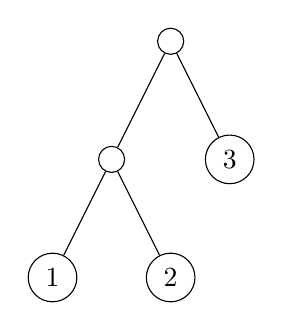
\begin{tikzpicture}
            \node [circle,draw] (z){$\orEff$}
                child { 
                    node [circle,draw] (a) {$\prEff$}
                    child { node[circle,draw] (b) {$1$} } 
                    child { node[circle,draw] (c) {$2$} }
                }
                child {
                    node [circle,draw] (d) {$3$}    
                };
        \end{tikzpicture}
        \hspace{2em}
        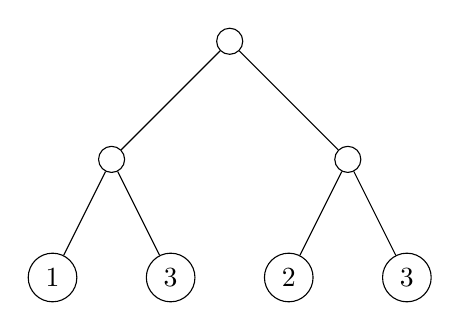
\begin{tikzpicture}[level 1/.style={sibling distance=3cm},
                            level 2/.style={sibling distance=1.5cm}]
            \node [circle,draw] (z){$\prEff$}
                child { 
                    node [circle,draw] (h) {$\orEff$}
                    child { node[circle,draw] (b) {$1$} } 
                    child { node[circle,draw] (c) {$3$} }
                }
                child {
                    node [circle,draw] (g) {$\orEff$}
                    child { node[circle,draw] (e) {$2$} } 
                    child { node[circle,draw] (f) {$3$} }
                };
        \end{tikzpicture}
    \end{center}
    \end{ensps}
    \begin{equation*}
        \orEff (\prEff (1,2), 3) \quad \quad \prEff (\orEff (1,3), \orEff (2,3))
    \end{equation*}
    \caption{The two trees from the counter example}
    \label{fig:counterexampletree}
\end{figure}

\begin{ensps}
We can see that the two trees in Figure \ref{fig:counterexampletree} 
have the same interpretation in terms of characteristic functions,
and the result from \cite{Mislove2000} shows us that a reasonable 
preorder shouldn't equate them. But we have an explicit 
cost function that shows that the interpretation in terms of 
expectancies is diffirent for the two trees:

\begin{equation*}
    h (i) = \begin{cases}
        1 & \text{ when } i = 1 \\
        8 & \text{ when } i = 2 \\
        2 & \text{ when } i = 3 \\
        0 & \text{ otherwise } 
    \end{cases}
\end{equation*}

This function can distinguish between the two trees 
because the least expected cost for the first one is $1/4$
where the least expected cost for the second one is $3/16$.

The choice of costs for $h$ is not random: we can divide 
everything by $8$ and build an actual substitution $\sigma$
such that $t_1 \sigma \not \equiv_{b} t_2 \sigma$, thus 
having an effective counter-example for the compositionality 
of the preorder.
\end{ensps}

Therefore,
this shows that for this preorder, \emph{compositionality
does not hold anymore}, even though 
it is still admissible. From a domain theoretic perspecitve,
we do have an embedding-projection pair with the domain 
of previsions using general functions, but the embedding 
is \emph{not} a homomorphism. Note that the exact same trees can be used 
as a counter example for the same claim in the case of angelic non-determinism. 
